\section{Architecture Générale}
\section{Préparation des données}
\section{Base de donnée}

\section{Interface avec le Reconnaisseur}

Cette partie du projet a pour objectif de lier la base d'apprentissage de notre logiciel avec le reconnaisseur choisi par l'utilisateur. Ainsi, cette partie étant très liée à l'utilisateur, il faut lui permettre de pouvoir facilement attacher le reconnaisseur de son choix au logiciel. C'est avec cette contrainte en tête que nous avons conçu l'architecture de cette partie.

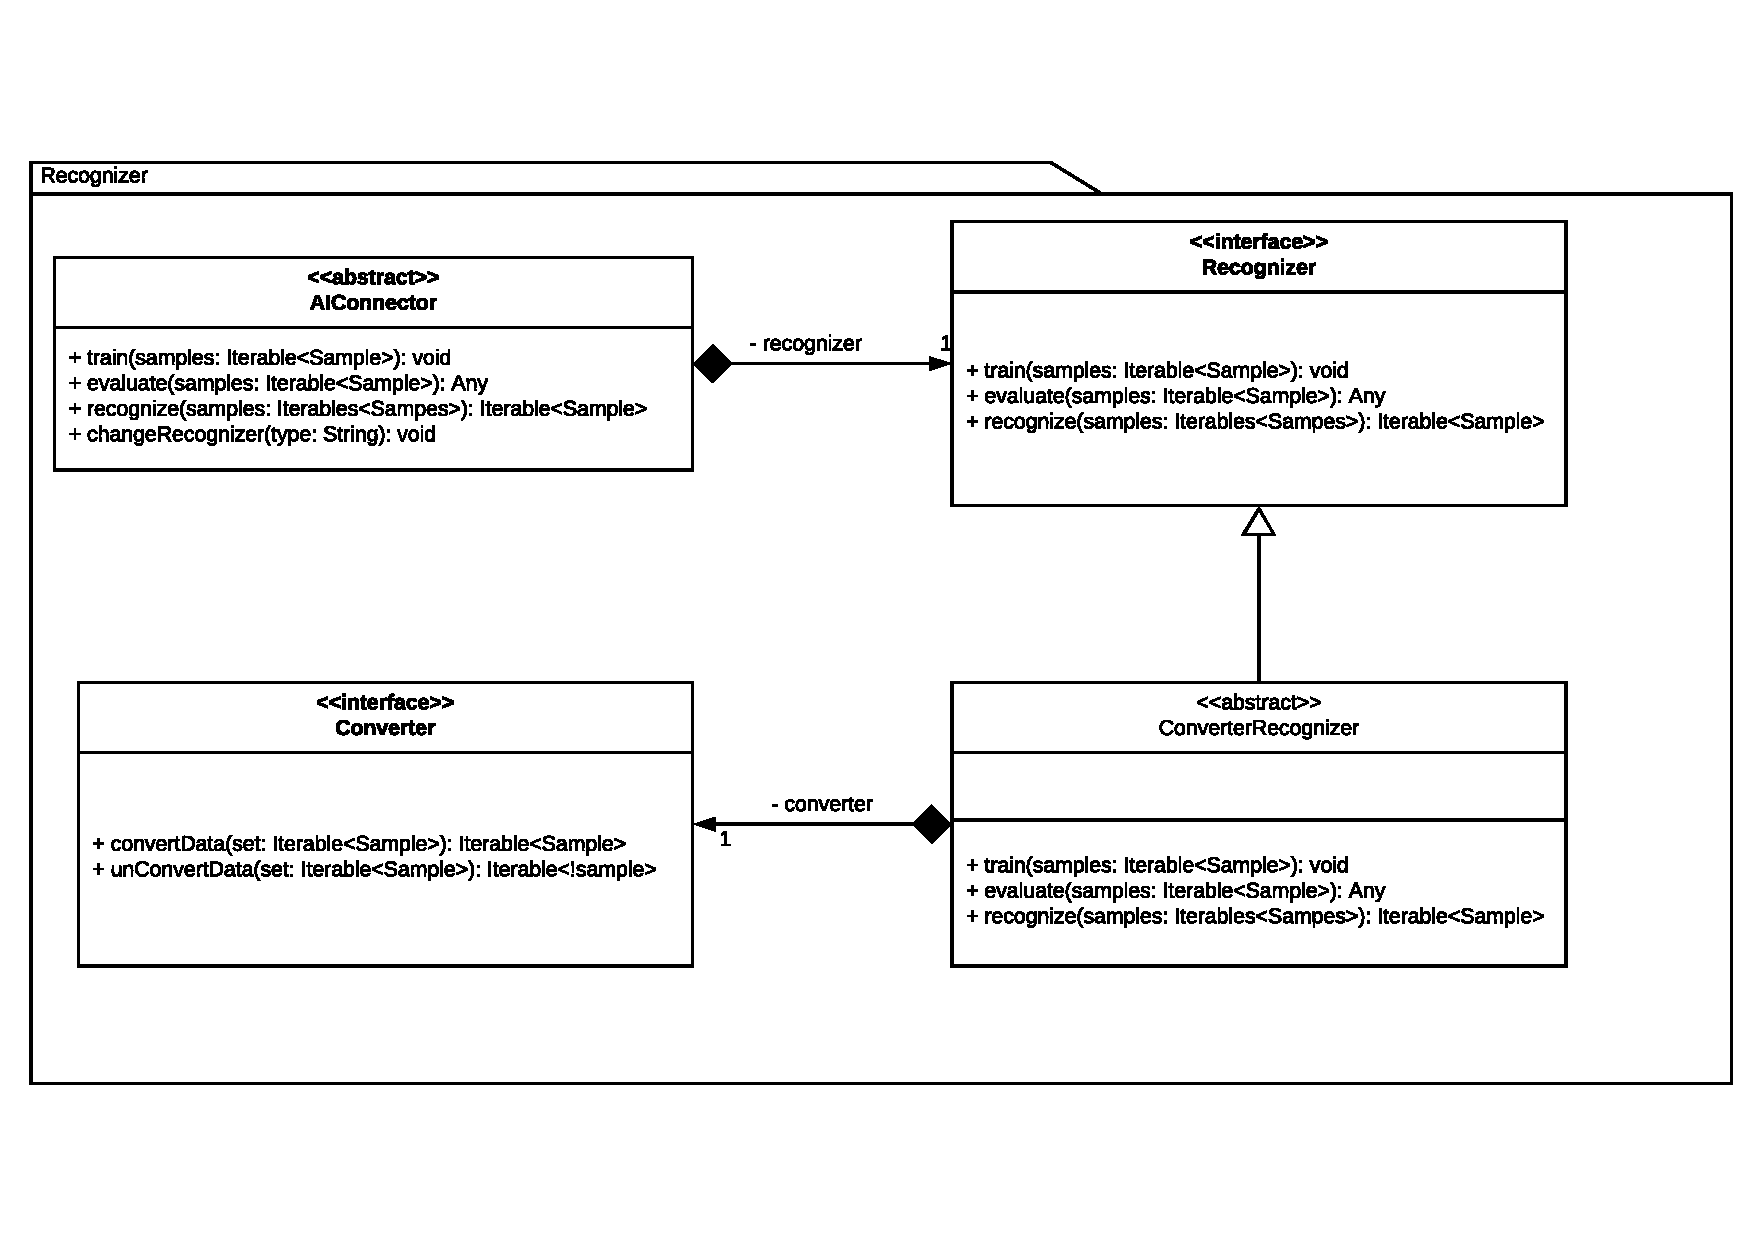
\includepdf[pages=-]{assets/UML_Recognizer}

\paragraph{Architecture}

Cette partie du projet contient comme toutes les autres un connecteur qui la lie au Connector principal. Ce connecteur possède un Recognizer afin de pouvoir effectuer les opérations classiques d'entrainement, d'évaluation de celui-ci ainsi que lui demander d'effectuer une transcription. Il permet également de changer de reconnaisseur quand l'utilisateur souhaite utiliser un autre type de reconnaisseur.
Le Reconnaiseur est représenté par une interface Recognizer qui permet trois actions possibles: entrainer le reconnaisseur à partir d'un ensemble d'apprentissage, évaluer ce même reconnaisseur sur un ensemble de validation, et enfin, lui demander de transcrire un ensemble non étiqueté.
Cette interface permet notamment à l'utilisateur, de connecter son propre reconnaisseur, et même s'il le souhaite, d'en créer un au sein de l'application. elle est également la seule qu'il est obligé d'implémenter pour faire fonctionner l'ensemble. Cependant, il faut dans certains cas convertir les données dans la base de donnée en données compréhensibles par le reconnaisseur. Ainsi, deux autres interfaces sont nécessaires: une interface Converter permettant la convertion des données entrantes et sortantes du reconnaisseur ainsi qu'une classe abstraite ConverterRecognizer héritant de Recognizer et possédant un convertisseur adapté au reconnaisseur utilisé.